\section{Interpolation-Based Compression: SZ3-HOHS}\label{sec:SZ3-HOHS}

In this section, we describe the interpolation-based prediction used in SZ3-HOHS. We first review the interpolation strategy in SZ3 as background, then introduce our modifications to adapt it to the non-uniform layout of HOHS data. Finally, we examine the effectiveness of cross-element prediction.

\subsection{Interpolation Prediction in SZ3}\label{sec:SZ3-HOHS:sz3 interpolation}

SZ3 employs a multi-dimensional prediction scheme, where the prediction of each data point is carried out along a particular dimension that can change from point to point. The compressor provides both linear and cubic interpolation predictors. In SZ3-HOHS, we focus on the linear interpolation predictor, which estimates each target data point using two reference points along a given dimension, due to its low computational cost.

For the linear interpolation in SZ3, as shown in Figure~\ref{fig:sz3 interpolation}, each data point is predicted using two neighboring values located at equal distances on opposite sides of the target point. The predicted value is computed as the arithmetic mean of these two references. This operation can be interpreted as fitting a linear function through the reference points and evaluating it at the target location. Owing to the symmetric placement of the neighbors, the prediction naturally reduces to their simple average.
Another situation involving two reference points arises as a boundary case of cubic interpolation, as illustrated in Figure~\ref{fig:sz3 interpolation}. Both reference points lie on the same side of the prediction target. In this case, the fitted model degenerates to a linear function defined by asymmetric reference positions, and the prediction becomes a weighted average rather than a simple mean.

\begin{figure}[htb]
    \centering
    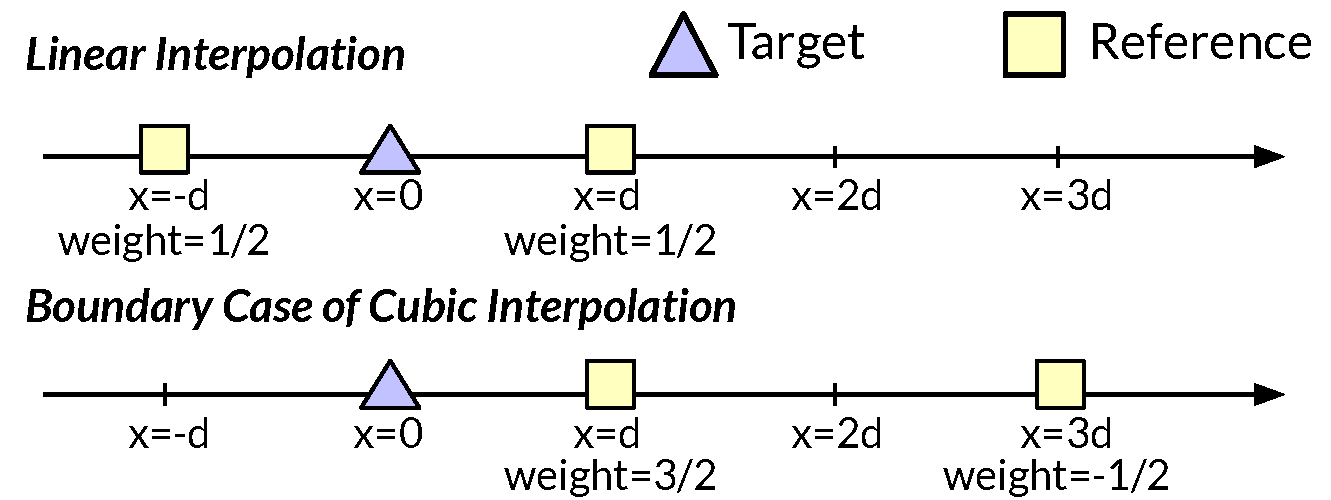
\includegraphics[width=0.9\linewidth]{figs/2-two-types-interpolation-in-sz3.pdf}
    \caption{Two Types of Interpolation in SZ3}
    \label{fig:sz3 interpolation}
\end{figure}

\subsection{Interpolation Prediction in SZ3-HOHS}

SZ3-HOHS extends the interpolation-based prediction strategy of SZ3 to accommodate the non-uniform spacing of data points in HOHS datasets. This adaptation involves two changes: distance-aware interpolation weights and a modified prediction order.

\begin{figure}[htb]
    \centering
    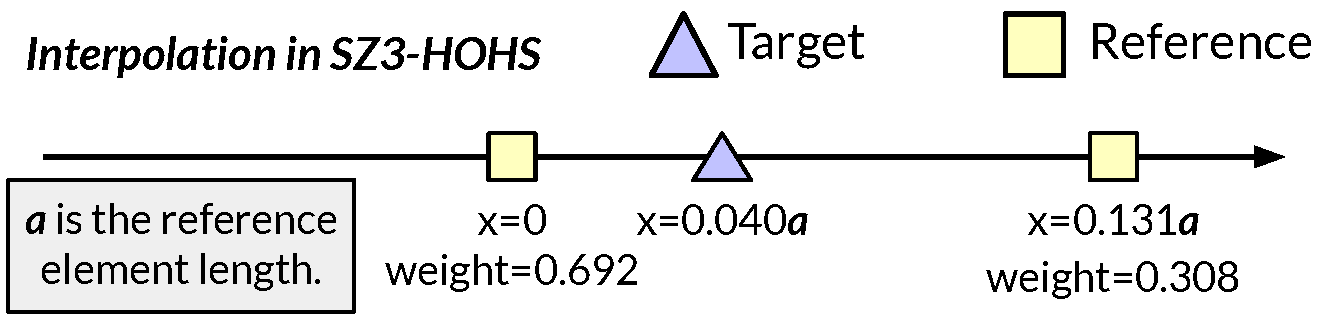
\includegraphics[width=0.9\linewidth]{figs/3-interpolation-in-hohs.pdf}
    \caption{Interpolation Method in SZ3-HOHS}
    \label{fig:sz3-hohs-interpolation}
\end{figure}

\begin{enumerate}
\item \textit{Distance-aware Interpolation Weights}: SZ3-HOHS adjusts the interpolation weights according to the relative physical distances between the prediction target and its reference points. Figure~\ref{fig:sz3-hohs-interpolation} shows an example of such non-uniform spacing. In this example, the distances from the target point to the closer and farther reference points are $0.040a$ and $0.091a$, respectively, corresponding to a distance ratio of approximately $1{:}2.26$, where $a$ denotes the length of the reference element. Accordingly, the closer reference point receives a larger interpolation weight, with the two weights being $0.692$ and $0.308$, respectively, corresponding to a weight ratio of approximately $2.26{:}1$.
\item \textit{Modified Prediction Order}: In SZ3, linear interpolation always chooses the data point located at the midpoint of the two reference points as the prediction target, where the notion of ``middle'' is well defined in both physical space and array index due to the structured layout of the data. In contrast, SZ3-HOHS selects the unpredicted data point closest to the physical center of the two reference points. This choice avoids overly extreme interpolation weights for the reference points, such as values close to 0 or 1. From a statistical perspective, it helps mitigate the propagation of compression errors from the reference points to the target.
\end{enumerate}

Another key observation of SZ3-HOHS is that, although physical spacing may vary across elements, the logical organization of data points within each element is fixed by the reference element and the associated GLL points~\cite{Isoparametric-Mapping}. Consequently, both the prediction order and the interpolation weights can be determined entirely from the reference element prior to compression. These prediction parameters are precomputed once and reused across all elements with the same polynomial order, eliminating the need for runtime distance calculations and ensuring negligible overhead.

In addition, SZ3-HOHS exhibits a slight performance advantage over SZ3 with respect to memory access behavior. When applied to large regular tensor datasets, SZ3 may involve long-range prediction accesses that can incur cache misses. In HOHS datasets, however, individual elements are typically small, often no larger than $10 \times 10 \times 10$, allowing SZ3-HOHS to operate primarily on cache-resident, element-local data.

\subsection{Evaluation of Cross-Element Prediction}\label{sec:SZ3-HOHS:cross_element}

\begin{figure}[htb]
    \centering
    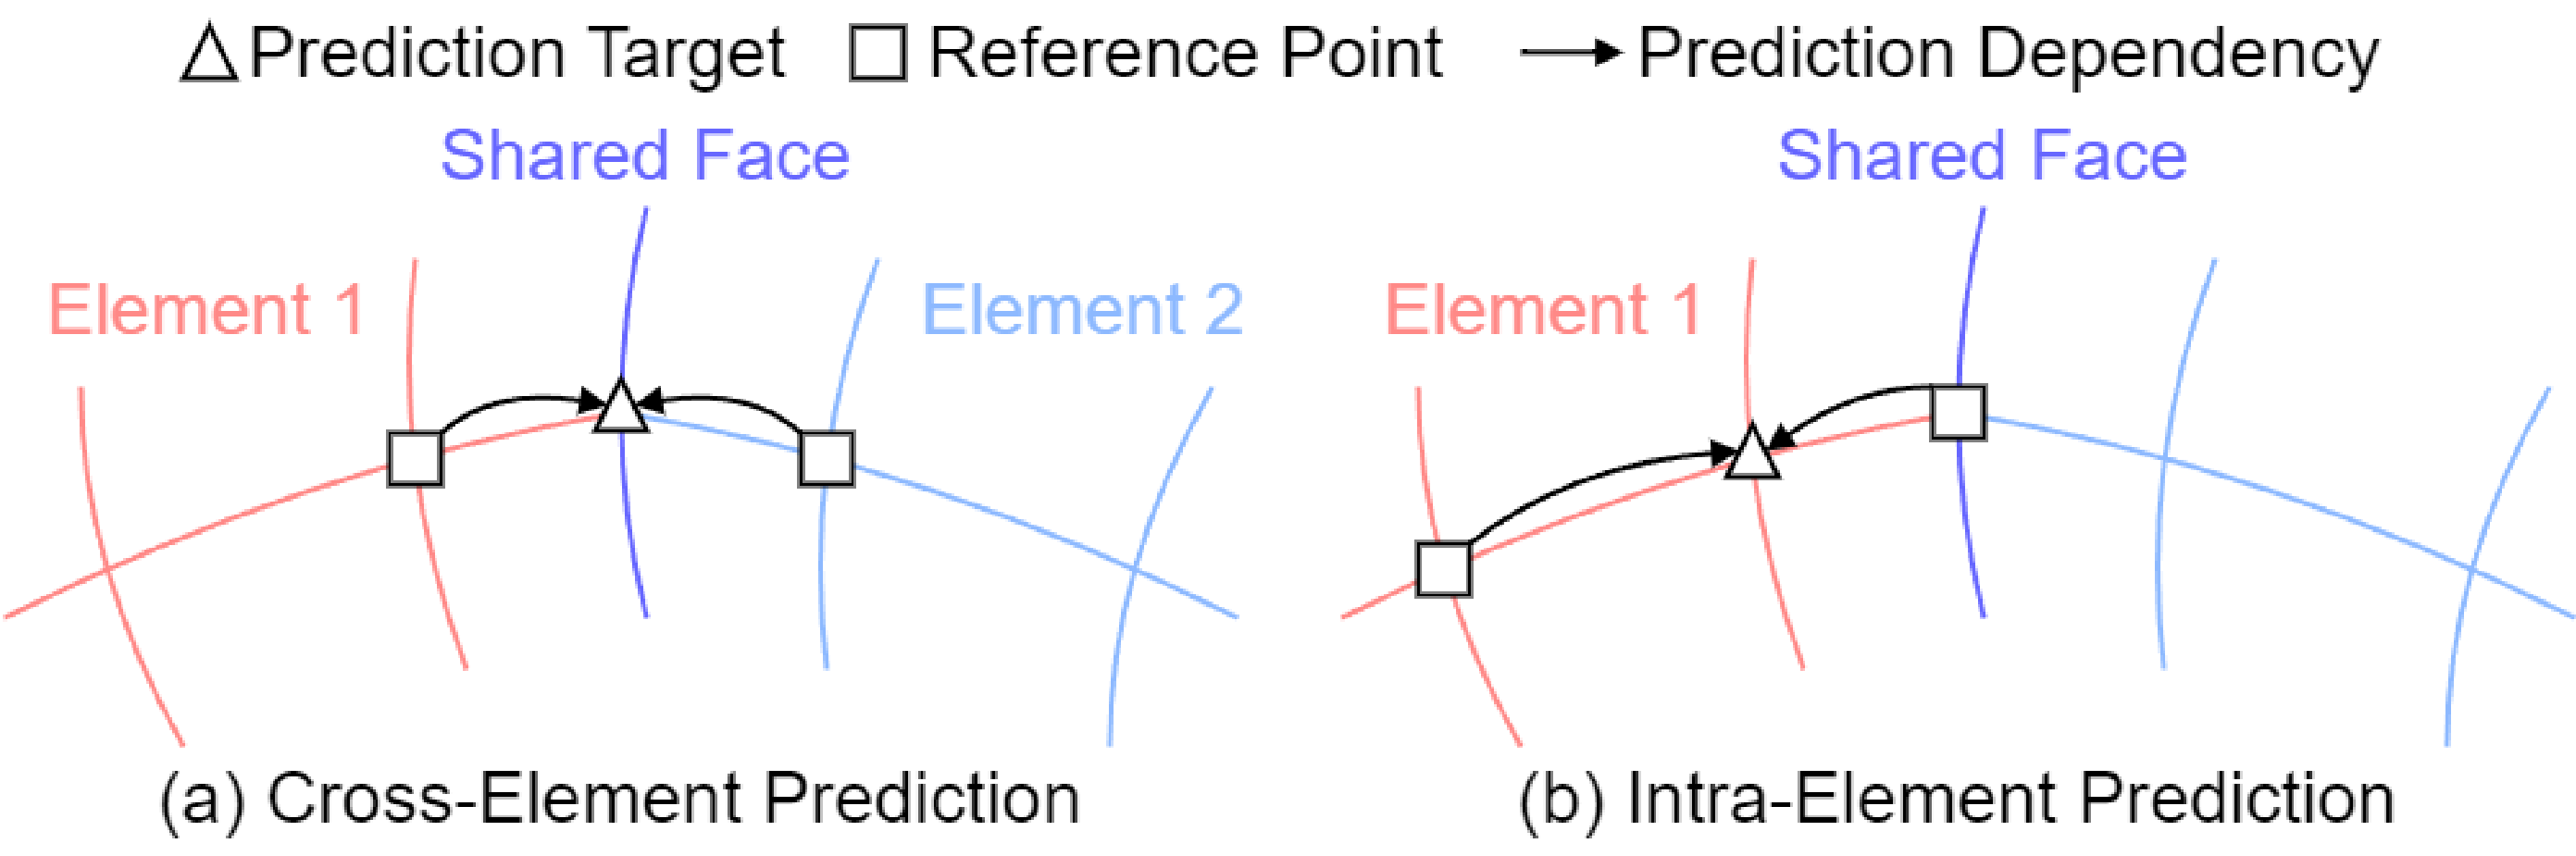
\includegraphics[width=1\linewidth]{figs/5/cross-element.pdf}
    \caption{Illustration of the Point Configurations Used in Cross-Element and Intra-Element Prediction}
    \label{fig:cross-element}
\end{figure}

We further explain the rationale for using intra-element prediction instead of cross-element prediction in SZ3-HOHS. In principle, cross-element prediction may benefit from the dense sampling near element boundaries. Since the physical distance between points across a shared face is small, their values may be more similar than those of neighboring points closer to the element interior, which can improve prediction accuracy. However, the reference points used in cross-element prediction are generally not collinear with the prediction target in physical space, which can reduce the effectiveness of linear interpolation. By contrast, the target and reference points used for intra-element prediction are collinear in the reference element and remain nearly collinear in physical space, with only minor distortion introduced by the element mapping. These competing effects make it unclear a priori which strategy provides more accurate predictions. We therefore perform an empirical comparison of cross-element and intra-element prediction.

We conduct experiments on the NekRS dataset~\cite{fischer2022nekrs} with an element size of $8\times8\times8$ (Dataset 4 in Table~\ref{tab:datasets}). We randomly sample a subset of elements, identify their neighboring elements, and align the neighboring elements to ensure consistent face orientations. For cross-element prediction, each point on the shared face is treated as a prediction target, and one neighboring interior grid point from each of the two adjacent elements is used as a reference for weighted linear interpolation. For comparison, the intra-element scheme predicts the same target using two reference points from the same element, both selected along the grid line extending from the shared face into the element interior. In both cases, prediction accuracy is quantified using mean squared error (MSE).

% \begin{table}[h]
%     \caption{MSE between cross-element and intra-element predictions across five faces of element 1940839.}
%     \label{tab:cross-element mse}
%     \centering
%     \begin{tabular}{c|cc}\toprule
%         \textbf{Adjacent Element} & \textbf{Cross-Element MSE} & \textbf{Intra-Element MSE} \\\midrule
        
%         1940803 & 2.049e-09 & 1.842e-08 \\
%         1940840 & 6.993e-04 & 1.146e-05\\
%         1940827 & 2.695e-07 & 3.909e-07\\
%         1940833 & 4.341e-08 & 2.526e-07\\
%         1940849 & 7.868e-06 & 1.031e-06\\\bottomrule
%     \end{tabular}
% \end{table}

\begin{table}[h]
    \caption{Comparison of Cross-Element and Intra-Element Prediction MSEs of a Representative Element}
    \label{tab:cross-element mse}
    \centering
    \begin{tabular}{c|cc}\toprule
        \textbf{Face Index} & \textbf{Cross-Element MSE} & \textbf{Intra-Element MSE} \\\midrule
        1 & 2.049e-09 & 1.842e-08 \\
        2 & 6.993e-04 & 1.146e-05\\
        3 & 2.695e-07 & 3.909e-07\\
        4 & 4.341e-08 & 2.526e-07\\
        5 & 7.868e-06 & 1.031e-06\\\bottomrule
    \end{tabular}
\end{table}

Table~\ref{tab:cross-element mse} presents the results for a representative element with five faces that have adjacent elements. Its remaining face has no identifiable adjacent element and is therefore excluded from the comparison. Additional tests show that either cross-element or intra-element prediction may achieve lower MSE on an individual face, while their average MSEs over a large number of faces are comparable. Thus, cross-element prediction provides no consistent accuracy advantage to justify the additional overhead of connectivity identification and orientation alignment. We therefore adopt intra-element prediction in SZ3-HOHS.